\documentclass[12pt]{article}
% $Id: bioperl-article.tex,v 1.17 2002-04-07 08:30:41 heikki Exp $
% $Log: not supported by cvs2svn $
% Revision 1.16  2002/04/06 19:07:08  lapp
% Spelled out GNF.
%
% Revision 1.15  2002/04/05 23:15:32  jason
% some changes to format towards GR - a few sentance reworks and transitions - cut it down to 5 main topics, pages for weblinks and each figure with captions
%
% Revision 1.14  2002/04/05 17:19:02  jason
% grammatical changes
%
% Revision 1.13  2002/04/02 00:07:13  jason
% rework, with Mark's comments - still need to add Matt's suggestions
%
% Revision 1.12  2002/03/25 14:17:28  jason
% small TeX bugs
%
% Revision 1.11  2002/03/24 20:49:13  jason
% reworking abstract, removed redundancy and greatly simplified the interoperability section.  Need to condense to probably 4-5 main sections
%
% Revision 1.10  2002/03/21 21:50:04  jason
% reworked abstract for GR and moved examples around.  Reworked abstract for GR and moved examples around.  Added statistics about tests and number of modulesTable for Modules rather than list.
%
% Revision 1.9  2002/03/19 10:58:47  heikki
% fixing examples, lot's of typos in the docs, minor changes
%
% Revision 1.8  2002/03/13 21:21:08  jason
% 3rd draft - with Lincoln's changes
%
% Revision 1.7  2002/03/04 22:18:09  jason
% Some reworking of text, placeholders for expansion on the major 
% theme of open-source developmentmore references and testing out 
% the lstlisting for code section, lines
% are not wrapping nicely though in 2-column mode with the code,
% Author list still incomplete and need to move acknowledgements
% around some more
%

\usepackage {listings,hyperref,url,apalike,layouts,
	     	epsfig,graphicx,keyval,fancyhdr,
	     setspace,fullpage }

\begin{document}

\doublespacing

\title{The Bioperl Toolkit: Perl modules for Biological Programming}
\author{Jason E Stajich$^1$ \and
Hilmar Lapp$^2$ \and
Heikki Lehv\"{a}slaiho$^3$ \and 
Lincoln D Stein$^4$ \and Ewan Birney$^3$ \and
Bioperl Project Team \thanks{Bioperl Mailing List bioperl-l@bioperl.org} \\
$^1$ \small{\textit{University Program in Genetics, Duke University,  Durham, NC USA}} \\
$^2$ \small{\textit{Genomics Institute of the Novartis Research
Foundation (GNF), San Diego, CA USA}} \\
$^3$ \small{\textit{European Bioinformatics Institute, Welcome Trust
Genome Campus, Hinxton, Cambridge UK}} \\
$^4$ \small{\textit{Cold Spring Harbor Laboratories, Cold Spring Harbor, NY USA }}\\
}
\maketitle
\begin{abstract}

The Bioperl project is an international open source collaboration of
biologists, bioinformaticians, and computer scientists that has
evolved over the last 7 years into the most comprehensive library of
Perl modules for manipulating and managing life science information.
Bioperl provides an easy-to-use, stable, and consistent programming
interface for bioinformatics application programmers.  The modules
have been successfully and repeatedly used to achieve otherwise
complex tasks with only a few lines of code.  The Bioperl object model
has been proven to be flexible enough to support enterprise-level
applications such as EnsEMBL, while at the same time keeping an easy
learning curve for novice Perl programmers.  Bioperl is also capable
of interoperating with other programming languages like Python and
Java through the evolving BioCORBA bridge and the accessing common
data storage through the BioSQL and Open Bioinformatics Database
Access projects.  The successful development of Bioperl depended in a
large part on the open source nature of the project.  We outline how
this approach is a valuable mechanism for collaborative projects.

[ Bioperl is available as open source software free of charge and
licensed under the Perl artistic license at \url{http://www.bioperl.org/}. ]

\textbf{Contact:} Bioperl project list \url{bioperl-l@bioperl.org}.

\end{abstract}

\section{Introduction}

Computational analysis is an integral part of modern biological
research.  Numerous computer software tools exist to perform 
data analyses, but it is not simple to automatically
combine data and results from multiple sources without the use of
computer software designed to read and write data specific to the
biological domain.  Bioinformatics consists largely of applying a
particular logic to this data integration.

One programming language, Perl, is by far the most widely used
programming language for these tasks, and is commonly thought of as
the language most easily grasped by newcomers to the field.  Perl has
been extremely successful for connecting software applications together into
sequence analysis pipelines, converting file formats, and extracting
information from the output of analysis programs and other text files.

Much of the Perl software in bioinformatics is specific to a
particular lab or institution and is not written in a general way so
that it can be used by others.  The Bioperl toolkit brings together
reusable Perl modules containing generalized routines specific to
biological and life science information.  A primary motivation behind
writing the toolkit is the authors' desire to focus energies on one
solution whose components could be shared rather than duplicating
effort.  In our minds, once a routine is written for parsing and
interpreting sequence from EMBL and Genbank format sequence files, no
one else should have to worry about writing their own.  In this spirit
we chose to make our code freely available and open source so that
others could contribute their solutions to the project as well.  Just
as the Human Genome Project was speeded and made more efficient by
public sharing of data, so has the open nature of the Bioperl project
reduced the time for solutions and new tools to reach the community
\cite{waterston}.

However, to be adopted by the community our software has to be user
friendly.  To that end we've both provided extensive documentation of
all the methods in each module, a graphical diagram of the objects in
the toolkit, and tutorials with examples of common problems.
Additionally we have written a module named Bio::Perl which provides
simple procedural functions  such as \textit{read\_sequence} which reads a sequence
from a file for users who do not want to study the entire module
hierarchy.  The goal of Bioperl is to help a user focus on their
specific problem at hand, such as the logic needed to process a BLAST
\cite{blast} report searching for hits that meet a certain species and
sequence length requirement, rather on than the actual mechanics of
\textit{parsing} that BLAST report.

\section{Methods}

The Bioperl project began in 1995 \cite{chervitz-bits} when there were
few programming toolkits for manipulating biological data or results
from sequence analysis programs.  Although Perl had already gained
widespread popularity in the bioinformatics community for its
efficient support of text processing and pattern matching tasks, there
were in fact no biological toolkits available in this language.

The project grew out of the following observations.  
\begin{itemize}

\item First, even though file formats of different analysis programs
are different, the information they represent is the same.  For
example, a pair-wise alignment is always between two sequences and has
common properties such as length, score, fraction of identities, start
and end of the aligned sequences, and so forth.

\item Second, the number of data structures needed to represent
information flow is limited, and common to most applications, such as
sequences, annotation, features, and alignments.  This permits a small
set of modules to be reused for variety of purposes and avoids
creating a confusing hierarchy of components.

\item Third, a set of operations is commonly performed on these data
structures.  These include reading and writing information to a file,
querying a sequence for its features, and translating a coding
sequence into protein.

\end{itemize}

This scenario naturally lends itself to the principle of
object-oriented programming, which Perl emulates with modules.
Object-oriented programming is the practice of grouping related tasks
together into logical and broadly applicable components such as a DNA
Sequence component which could contain methods such as retrieve the
accession number, reverse complement, or translated protein sequence.
The mission of Bioperl is to provide an easy-to-use object-oriented
Perl library that contains data structures and operations commonly
used in the life sciences ain clean, generic, and re-usable modules.
By separating the components into logical groups, such as sequences,
alignments, and databases, we have been able to add features to a
specific module without necessarily affecting the rest of the toolkit
library.  This separation is a key component of object-oriented
programming and permits us to produce generic components which can be
used for multiple purposes.  

At present the objects and operations in Bioperl center around
biological sequence analysis and annotation.  In the last year the
project has expanded to address new areas including phylogenetics,
maps, protein structure, and bibliographic references.  The project
has over 300 modules and comprises more than 160,000 lines of code and
embedded documentation.  The Perl modules are organized by logical
names so that, for example, the Bio::Search hierarchy contains modules
related to database searches and Bio::Graphics contains modules that
are related to drawing.

When designing Bioperl objects our objective was to provide a
programming interface that is very easy to use but that at the same
time could be easily extended in its capabilities and behavior through
code reuse.  Using an object-oriented paradigm we followed certain
design principles.

\begin{itemize}

\item Separating the interface from the implementation.  The key
information about an object class is the method names and their list
of accepted arguments.  Interfaces are collections of methods which
describe the expected behavior of a module, but do not do any of the
work.  Child classes inherit from the interfaces and are specialized
instances of their parents to perform specific tasks.  For example the
sequence parsing factory class Bio::SeqIO describes methods
\textit{next\_seq} and \textit{write\_seq} which are implemented 
differently by the child classes Bio::SeqIO::genbank and
Bio::SeqIO::embl for reading and writing their specific sequence data format.

\item Generalize common routines into a module.  When many modules
follow the same route to accessing data it is useful to group those
routines together.  A good example of this is data Input/Output (IO).
A top-level IO object called Bio::Root::IO was created to manage basic
access to files and data streams.  Because all modules that need data
access use operations from the IO module access to data is consistent
across the entire package. It is also ease share any enhancements to
the common methods because any changes made in the parent module will
be inherited by the child modules.  Figure 1 shows a schematic of how
2 modules which have different tasks inherit from a single IO module
which provides a function that is shared.

\end{itemize}

In Bioperl we followed these two design patterns \cite{gangoffour}
wherever possible.  To help distinguish implementation classes from
interface definition we used a capital 'I' appended to the object
name, e.g., the interface Bio::SeqI and its implementing class
Bio::Seq.

Bioperl is written purely in Perl and depends on at least version 5.005
of the Perl interpreter.  The toolkit has been checked
for cross-platform compatibility on most UNIX and UNIX-like operating
systems in addition to Macintosh OS X and Microsoft Windows operating
systems.  Since the toolkit is run through the Perl interpreter,
specific issues are often due to compatibility between different
versions of Perl.  Descriptions of specific bugs and their solutions
are available from the Bioperl website.

In addition to pure Perl solutions to bioinformatics problems, Bioperl
can take advantage of external data analysis packages.  Currently the
toolkit supports interactions with applications in the EMBOSS
\cite{emboss} suite, NCBI BLAST, and the multiple sequence alignment
programs ClustalW \cite{clustalw} and T-Coffee \cite{tcoffee}.  In
some cases, when an external package is not available, Bioperl will
fall back to using a slower method, either by emulating the package in
pure Perl or by invoking a network-based analysis service such as the
NCBI BLAST analysis queue.  Additional work is in progress to
incorporate into the project access to remote analysis services at the
European Bioinformatics Institute and Pasteur Institute.

In order for us to produce fairly uniform software code, we established
coding guidelines that are extensions of good object-oriented
programming.  All modules were required to meet minimal standards
before releasing.  These standards included a complete set of
regression tests, well formed embedded documentation for each method,
and a concise example code in the SYNOPSIS section of each module's
documention.  The Perl embedded documentation format (called POD, or
Plain Old Documentation) is used to provide annotation within the
source code.  This documentation can be converted to text, TeX, or
HTML.  We have used the Pdoc \url{http://pdoc.sourceforge.net} tool to generate colored and
organized documention in HTML for easy online browsing.

The development process involves integrated testing of the code.  We
accomplished this by insuring that each module has a test in the
Bioperl test system.  This approach is effective in locating newly
introduced bugs and is a tenent of the Extreme
Programming\cite{xprogramming} methodology.  The Extreme Programming
approach is to build the test for a module first and implement the
module which completes the test second.  This approach insures that
all tested aspects of the module's implementation were correctly
completed successfully.  The Bioperl 1.0 release has over 3000 tests
which assists in insuring the quality of the source code releases and
checks that new changes to the code do not break the
expected behavior of modules.

To support multiple developers in different time zones and
institutions, a centralized repository for the source code for the
project was setup in Boston, MA.  The Open Bioinformatics Foundation
(OBF) was founded, in part, to assist in the ownership and management
of the servers which contain source code repositories and websites for
a collection of open source bioinformatics toolkits.  Using a software
development tool called Concurrent Version Control system
(\url{http://www.cvshome.org}) \cite{cvsbook} multiple developers can work on the software source
code at the same time and commit their changes into a central
repository without having to communicate.  The ability to share code
easily and quickly is one of the primary building blocks in
establishing a successful open source project.

\section{Results}

Bioperl has 10 active developers led by a core of 5 primary developers
who insure that standards are met, prepare code releases, and set the
vision for the project.  The mailing lists for the project include
1300 subscribers and about 10,000 unique visitors to our website each
month.  The project has been used in variety of endeavors including
genome sequencing, annotation, sequence variation elucidation, disease
gene discovery, and comparative genomics.

By far the most advanced use of the Bioperl toolkit has come through
the EnsEMBL\cite{ensembl-nar} project.  The basic sequence handling,
file format parsing, and sequence features for annotation model have
been used as building blocks for automatically annotating the
\textit{Danio rerio}, \textit{Drosophila melanogastor}, \textit{Fugu
rubripes}, \textit{Homo sapiens}, and \textit{Mus musculus} genomes (\url{http://www.ensembl.org}).

Additionally the Genquire\cite{genquire} annotation package makes use
of the Bioperl object model and stores sequence and annotation data in
a persistent database model.  The sequence rendering capabilities are
partitioned into a specific Bioperl package called bioperl-gui.  The
database model used by Genquire has been updated to utilize the
Open Bioinformatics Database Access (OBDA) (\url{http://obda.open-bio.org}) sequence database design, which
will allow the other OBF toolkits to access data written by the
Genquire system.

The Generic Model Organism Browser (GMOD) \cite{gmod}, Distributed
Annotation System Perl (DAS) server \cite{das}, and TFBS
\cite{tfbs} all use the Bioperl object model to describe sequences and
Bioperl tools to complete analyses.  The GMOD system is a web
interface to databases of features for a genome project.  The DAS
system provides researchers a means to locally annotate sequences and
publish the annotations to the community via the DAS XML protocol.
TFBS provides a perl implementation of objects for DNA sequence pattern
representation by matrix profiles, with associated methods for searching
the sequences for the occurence of patterns, pattern storage, and
generation of new patterns. The implementation uses Bioperl sequence,
alignment, sequence feature and feature pair objects.

\subsection{Interoperability}

Sometimes the best solution for a bioinformatics problem is a hybrid
of multiple tools.  These tools, written in different programming
languages such as C, Java, and Python, can be used within a Perl
script simply by invoking them (a process often called ``shelling
out'').  In some situations these tools require that data be available
in a certain format or within a certain database.  Bioperl provides
software layers which can, for example, populate a database with
sequence information which can be accessed and used to generate an
interactive graphical interface provided by the Biojava toolkit.
In other cases, Bioperl is used to create files in a format recognized
by other programs so that they can perform their analyses. 

The Extensible Markup Language (XML) provides a means for creating
data in a language and platform independent manner.  Previous work has
outlined scenarios where XML has been useful in a biological context
\cite{xmlbioinformatics}.  Bioperl supports several XML standards for
biological data including BSML (read only) and GAME (read/write)
sequence markup formats.  Bioperl can parse NCBI BLAST XML format in
addition to the standard BLAST text format.  It also supports Medline
XML (read only) provided by the European Bioinformatics Institute's
Bibliographic Query Service (BQS) and Entrez Pubmed XML format.

The Common Object Request Broker Architecture (CORBA)
allows a programmer to share components developed in different
languages.  This is achieved by first agreeing upon the names of
functions and data the components will contain.  Developers write the
software for the components in their favorite language and run a
program called a server where the components can be accessed from.  A
simple example of this is a component to retrieve sequences from a
database.  It is written in the Perl and is loaded into a server
program.  A programmer will then write software in Java which connects
to the server program and requests a specific sequence by its
accession number.  The Perl component will do its job and find the
sequence and return it to the Java program.  By using these types of
building blocks, larger and more complex bioinformatics solutions can
be built which can maximize the strengths of various programming
languages and environments.  An example of a proposed standard for
CORBA components for biological processes is the BioCORBA
(\url{http://www.biocorba.org}) project.  It is a collaborative
project which has involved members of the Bioperl, Biojava
(\url{http://www.biojava.org}), and Biopython
(\url{http://www.biopython.org}) projects as well as the Object
Management Group's Life Science Research group
(\url{http://lsr.ebi.ac.uk}).

This interoperability has also been applied to the EnsEMBL project.
The EnsEMBL (v. 4) software layer is a collection of Perl modules
built on top of the Bioperl library.  Using an EnsEMBL-CORBA interface
derived from BioCORBA, a Perl EnsEMBL CORBA server has been written
which is accessible to C, Java, and Python clients, and therefore
making the EnsEMBL data and algorithms programatically available to
these languages.

\section{Conclusions}

In the future, Bioperl will continue to evolve in order to address
more issues in bioinformatics.  We plan to create objects to
manage sequence assembly information, haplotype maps, gene expression,
and protein interaction data.  Additionally, projects focusing on
multi-species comparisions are building Perl modules to manage the
alignment and syntenic information.  We are creating software layers
to interact with OBDA databases, developing an analysis pipeline
system to provide automated annotation, and expanding the supported
file formats the toolkit can read and write.

Much of the success of the Bioperl toolkit development effort can be
attributed to the Open Source nature of the development effort which
has allowed a diverse group of individuals to participate in
collaborative project.  By encouraging users of the toolkit to also
assist in the development of it, contributions are made back to the
source code base which can benefit all users.  This collaborative
effort and the strong need to get working software written in
an extensible manner has made Bioperl an excellent platform for Perl
bioinformatics software development.  This open sharing of ideas that
embodies the scientific spirit is successful in the world of software
development for scientific purposes as well and has permitted the
toolkit to grow in directions pertinent to its users.

\section{Acknowledgements}

The Bioperl Core is Jason Stajich, Hilmar Lapp, Heikki Lehv\"{a}slaiho,
Lincoln Stein, and Ewan Birney.  The project has seen signifigant
contributions from the following people: David Block, Kris Boulez,
Steven Brenner, Brad Chapman, Steve Chervitz, Michele Clamp, Tony Cox,
James Cuff, Chris Dagdigian, Andrew Dalke, Allen Day, Arne Elofsson,
Mark Fiers, Georg Fuellen, James R Gilbert, Ed Green, Roger Hall,
Peter van Heusden, Joseph Insana, Nicolas Joly, Ian Korf, Aaron J
Mackey, Brad Marshall, Chad Matsalla, Chris Mungall, Emmanuel Mongin,
Brian Osborne, Lorenz Pollak, Matthew Pockock, Todd Richmond, Martin
Senger, Peter Schattner, Elia Stupka, Gert Thijs, Charles Tilford,
Andrew Walsh, Kai Wang, Mark Wilkinson, and Alex Zelensky.

Additional ideas and help came from other OBF project team members
including Jeff Chang, Thomas Down, Keith James, and all of the Bioperl
mailing list members.

We would like to especially acknowledge Steve Chervitz for his
previous role as Bioperl project leader.  Thanks also to Brian Osborne
and Peter Schattner for their excellent documentation and tutorial
work, and Chris Dagdigian for his tremendous support as system
administrator for the project computers.

The Bioperl project and its sister projects (commonly referred to as
the Bio\{*\} projects) are supported under the umbrella of the Open
Bioinformatics Foundation (OBF) \url{http://www.open-bio.org}.
OBF is supported by hardware donations from Compaq and Sun
Microsystems, and we graciously accept donated bandwith and computer
server space from Wyeth.

J.E.S is supported by an NIH Genetics training grant.  Thanks to
F.Dietrich, M.DeLong, M.Hahn for their comments on this manuscript.

\bibliography{bioperl}
\bibliographystyle{apalike} 

\newpage

\section{Website References}

\url{http://www.biocorba.org}, BioCORBA Project. \\
\url{http://www.biojava.org}, Biojava Project. \\
\url{http://www.biopython.org}, Biopython Project. \\
\url{http://www.cvshome.org}, CVS Home Page. \\
\url{http://www.ensembl.org}, EnsEMBL Project Home page. \\
\url{http://obda.open-bio.org}, Open Bioinformatics Data Access. \\
\url{http://www.open-bio.org}, Open Bioinformatics Foundation. \\
\url{http://lsr.ebi.ac.uk}, Object Management Group's Life Science Research group. \\
\url{http://pdoc.sourceforge.net}, Pdoc Home Page. \\
\url{http://forkhead.cgr.ki.se/TFBS/}, TFBS Project. \\

\newpage 

% for right hand top labels

\pagestyle{fancy}
\fancyhf{}
\renewcommand{\headrulewidth}{0pt}

\rhead{Stajich\_Table1}

\begin{table}[h]
\begin{tabular}{|l|l|}
\hline
\textbf{Modules} & \textbf{Description} \\
\hline
Bio::Seq &  Sequences and their properties \\
Bio::SeqIO & Sequence data input/output \\
Bio::Index & Local sequence database indexing and retrieval \\ 
Bio::DB & Remote database access for sequences and references via HTTP \\
Bio::DB::GFF & Local GFF database for DAS and GMOD \\
Bio::SeqFeature & Feature representation and annotation \\
Bio::Annotation & Generic annotation \\
Bio::AlignIO, Bio::SimpleAlign & Multiple alignment representation \\
Bio::LiveSeq, Bio::Variation & Sequence variations and mutations \\
Bio::SearchIO, Bio::Search  & Sequence database searches and their Input/Output \\
Bio::Tools &  Miscellaneous analysis tools \\
Bio::Tools::Run &  Wrapper for executing local and remote analyses \\
Bio::Tree, Bio::TreeIO & Phylogenetic trees and their Input/Output  \\
Bio::Structure & Protein structure data \\
Bio::Map, Bio::MapIO & Biological maps and their Input/Output \\
Bio::Biblio, Bio::DB::Biblio & Biblopraphic References and Database
retrieval \\ 
Bio::Graphics & Graphical displays of sequences \\
\hline
\end{tabular}
\caption{Major Bioperl module groups}
\label{modules}
\end{table}

\newpage

\rhead{Stajich\_Figure1\_caption}

Figure 1.  Object-oriented inheritance of the readline() method to the
Sequence Reader and Report Reader modules from the IO class module
illustrates how shared functions can be aggregated and reused.

\newpage

\rhead{Stajich\_Figure2\_caption}

Figure 2. Sequence retrieval from the Remote GenBank Database at EMBL.
This code retrieve an mRNA sequences from the EBI EMBL databank with
the accession number U14680 and write the sequence out in GenBank
format to the screen.  One could replace Bio::DB::EMBL with
Bio::DB::GenBank and instead retrieve the sequence from NCBI.

\newpage

\rhead{Stajich\_Figure3\_caption}

Figure 3. BLAST parsing. A BLAST report is parsed and only hits meeting
an e-value and length threshold are saved in the array @HitsToSave.  
In this case any hit with evalue greater than 0.001 or length less 
than 120 residues will be excluded.  Once the list of hits is built 
one can print out the name of each of the Hits which had High Scoring
Pairs (HSPs) that met the criteria

\newpage

\rhead{Stajich\_Figure1}

\centerline{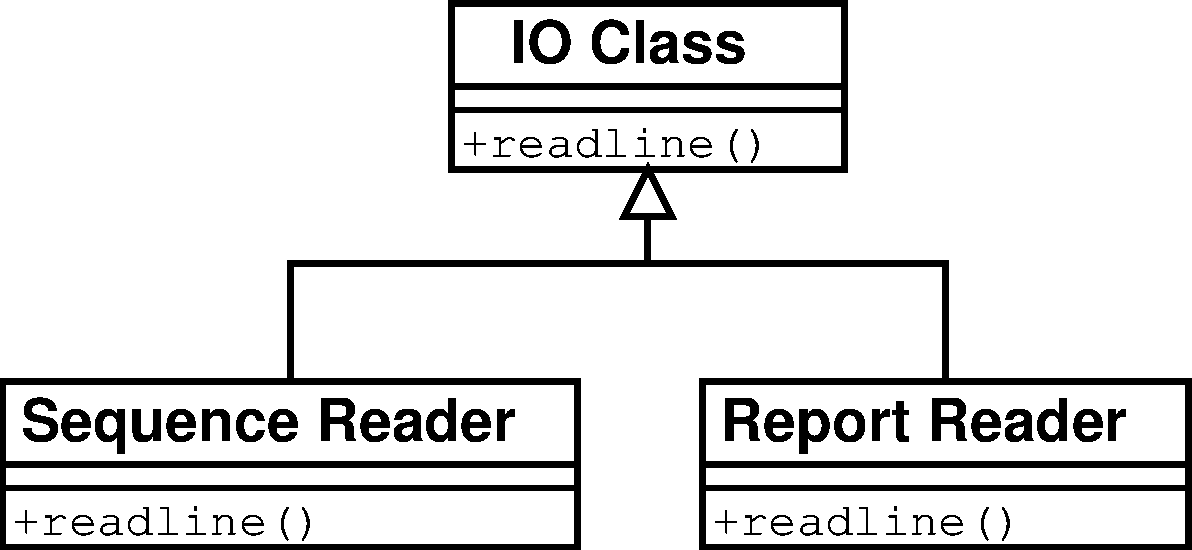
\epsfig{file=oo_inheritance}}

\newpage

\singlespacing

\rhead{Stajich\_Figure2}

\lstset{
	language=Perl,
	basicstyle=\small,
%	labelstyle=\tiny,
%	labelstep=1,
	stringstyle={} }

\begin{scriptsize}
\begin{lstlisting}{}
use Bio::DB::EMBL;
use Bio::SeqIO;

my $db = new Bio::DB::EMBL();
my $seq = $db->get_Seq_by_acc("U14680");
my $seqout = new Bio::SeqIO(-format => "genbank");
if (defined $seq) { # in case DB doesn't return anything
    $seqout->write_seq($seq);
}
\end{lstlisting}
\end{scriptsize}

% $

\newpage

\rhead{Stajich\_Figure3}

\begin{scriptsize}
\begin{lstlisting}{}
use Bio::SearchIO;
# Let's parse a BLAST report 
my $search = new Bio::SearchIO(-format => 'blast',
          		       -file   => 'report.bls');
my @HitsToSave;
my $cutoff_Evalue = 0.001; # max e-value is 0.001
my $cutoff_Len   = 120;    # min length of 120 residues
while(my $result = $search->next_result) {
 HIT:while(my $hit = $result->next_hit) {
   while( my $hsp = $hit->next_hsp ) {
    if( $hsp->evalue < $cutoff_Evalue && 
	$hsp->length('total') >= $cutofflen ) { 
	push @HitsToSave, $hit;
	next HIT;
      } 
   }
  }
}
# process hits that meet criteria
print "Hits:\n";
foreach my $hit ( @HitsToSave ) {
  print $hit->name, "\n";	
}

\end{lstlisting}
\end{scriptsize}

\end{document}
